\section{Choice of Hardware \& Software}\todo{What is this section supposed to be about? What already decide upon our hardware and software in the chapter about analysis, and the chapter about design.}

\subsection*{Hardware}
\todo{Put a couple of pictures from different angles of the bus here.}


\subsection*{Software}
As for writing software for the NXT, it has been decided that the program is being written using nxtOSEK. C and C++ are both very powerful low-level languages, and it has a scheduling system that allows us to more easily plan how the program should prioritise. These played a big role in this decision. Not only that, the option to use the NXT BIOS reduces the chance of memory issues, which might occur once the program starts growing in functionality.

\subsubsection*{NOTICE}
Fix position and order of below content, also make it be more fluid. basically fix everything

\subsubsection*{Input / Output}
The NXT has 3 outputs and 4 inputs. The inputs are named alphabetically, A to C. Where the inputs are numerically, 1 through 4. In addition to this, it has USB and Bluetooth connectivity.

\begin{figure}[H]
    \label{software_nxtbrick}
    \centering
    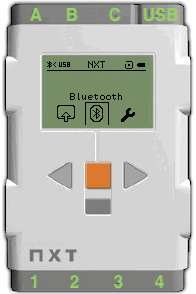
\includegraphics[width=0.4\textwidth]{Images/Software/NXT/nxtbrick.png}
    \caption{The I/O of the brick}
\end{figure}

Furthermore there are 4 physical buttons on the device. However using nxtOSEK only the middle and right button can be used, as the bottom button is used for shutting off the device, and the left button is used for going back to the BIOS.

\subsubsection*{Motors}
The motors use Pulse Width Modulation\info{Do we talk about this elsewhere?}, shortened PWM, to control the speed. PWM is based on pulses of a fixed length, within these, the amount of time that it is high creates a percentage.

\begin{figure}[H]
    \label{software_duty_cycles}
    \centering
    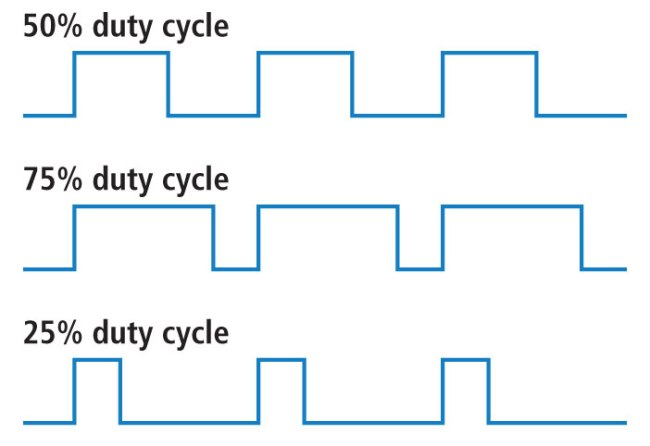
\includegraphics[scale=0.8]{Images/Software/NXT/duty_cycle.jpg}
    \caption{Example of duty cycles\todo[inline]{Do we know the frequency?}}
\end{figure}

If it is high during the entire duration it translates to 100\%. This means that the output of the motor is given on a percentage basis.

The motor can furthermore return values, in which it is important to understand that the engine is a stepper motor, its precision is for each degree it has turned. Meaning that if we receive a value of 360, it has turned an entire cycle. The direction is also given, by returning either a negative or positive value.

\subsubsection*{Camera}
The NXTCam can connect using both USB and LEGO cables. Using the LEGO connector requires the use of the I2C protocol.
To select line tracking mode, send 0x4C. X to disable sorting\todo{Make this make sense + fix char / hex}. It returns 78 if a configuration error has occurred. Ex. not sending sorting config creates config error.

\subsubsection*{LCD}
The display can be useful for showing any debugging information, although noteworthy is that the 100x64 pixel display is a fairly limited size. The display uses a double buffering system to avoid rendering partials. The display command takes 16ms for it to appear on the display.

When there are suddenly masses of data that can be relevant for debugging, communicating to a host can be more useful.

\subsubsection*{Host Communication}
The NXT supports communication via the USB port or Bluetooth using the bluecore chip.

\subsubsection*{Packets}
USB communication supports packets up to a size of 64 bytes, where Bluetooth supports 256 bytes for transfers and 128 bytes when receiving. As it can be convenient to support both systems without further changes, the common denominator of 64 has been chosen.

The host sends a packet that indicates which type of data it needs. The slave, in this case the NXT, returns a set of data. Noteworthy is that if one is to send multiple packets from one end, sending acknowledgement packets, similar to what TCP does, is recommended, Otherwise, data can be lost or errors might occur.
It is structured such that the initial byte indicates the number of objects given, whereafter it proceeds to give the data in the next elements. While the NXTCam returns its lower right X and Y coordinates, it is deemed unnecessary overhead as it is easily calculated by the width and height.

\begin{figure}[H]
    \label{software_packet_cam}
    \centering
    
\includegraphics[width=0.8\textwidth]{Images/Software/NXT/packet_cam.png}
    \caption{Packets structure of cam data transfer.}
\end{figure}

\todo{Short introduction of what the USB connection/Bluetooth connection is for.}In figure \ref{software_packet_cam} the initial byte is the number of objects, followed by the X and Y coordinates, width, height and colour of the n-th object. The colour is a value between 1 and 8 which is based on the colormaps. 
The camera only tracks 8 elements, meaning that with 5 elements per object, it uses $5 * 8$ elements, meaning that the camera objects occupy 40 bytes, where it is important to remember the first element that counts the number of objects. Meaning that it uses 41 out of 64 available bytes.
This leaves room for monitoring other factors, such as the turning angle.

If one is to send numbers of greater length than can fit within a byte, splitting the digit of the number into different bytes can be performed.
